\documentclass{beamer}
  \usepackage[utf8]{inputenc}
  \usetheme{Warsaw}
  \graphicspath{images/}
  \usepackage{amsmath} 
  \usepackage{amssymb}

  \title{Are New Technologies an issue for society?}
  \author{Clément CAUMES \& Mehdi MTALSI-MERIMI}
  \institute{UFR des Sciences Versailles - M1 Informatique}
  \date{Semestre 2} % RAJOUTER PLAN ICI

  \begin{document}

\section{Introduction}

  \begin{frame}
  \titlepage
  \end{frame}

\section{A curb for our planet}

\subsection{Destroy resources}

 \begin{frame}
\begin{block}{Issues of resources} 
	Increase of population, demands and productions induce :
	\begin{itemize}
		\setbeamertemplate{itemize item}[circle]
		\item Resource overexploitation
		\item Extinction of rare animals and plant species
	\end{itemize}
	\hspace{2.5cm}
	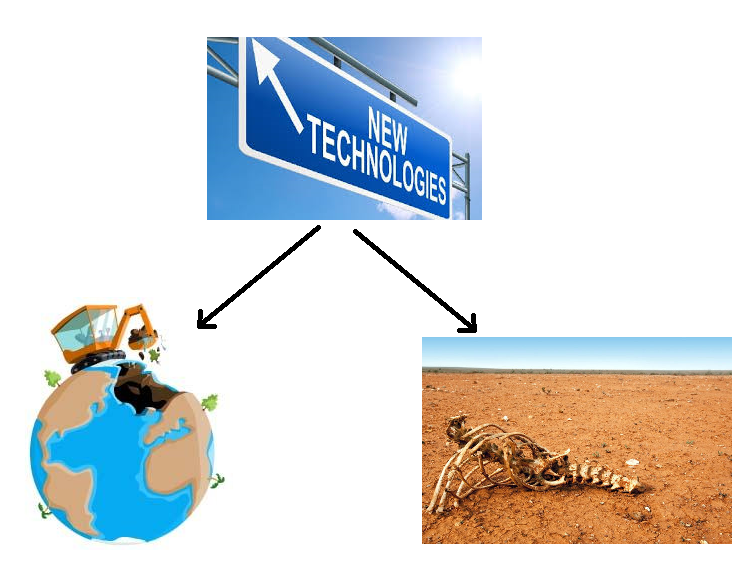
\includegraphics[scale=0.3]{pics/image1.png}
	\end{block}
\end{frame}

\begin{frame}

\begin{block}{Date of exhaustion of mineable resources} 
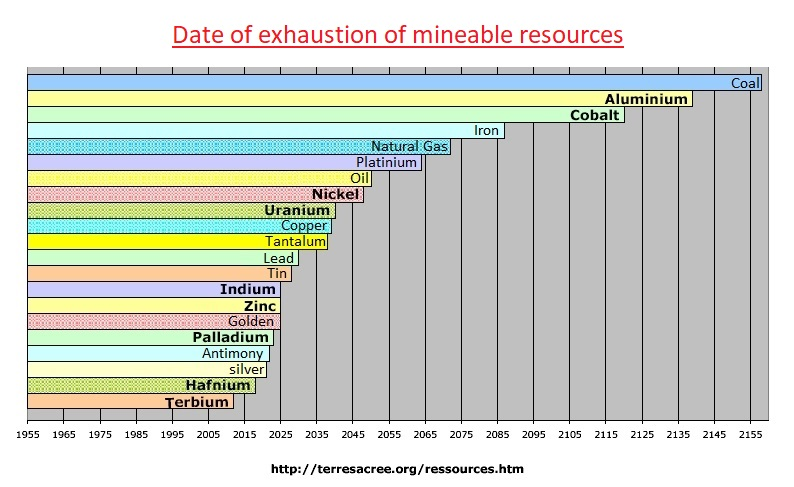
\includegraphics[scale=0.45]{pics/image2.jpg}
\end{block}

\end{frame}

\subsection{Contribute to the pollution}



\section{An impact for a social perspective}

\subsection{Increase addictions}

\subsection{Creating Inequalities}

\subsection{Creating Conflicts}

\section{Conclusion}
    
  
  \begin{frame}
  \hspace{5cm}
  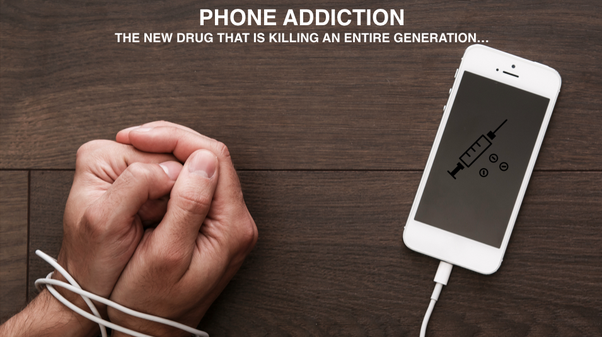
\includegraphics[scale=0.7]{ANGS3/addiction.png}
  \end{frame}
  
  \begin{frame}
  \hspace{5cm}
  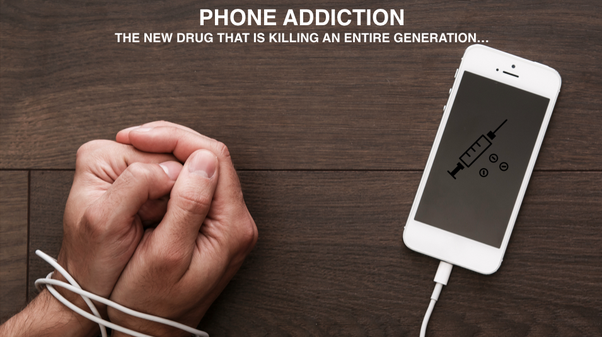
\includegraphics[scale=0.7]{ANGS3/addiction.png}
  \end{frame}
  
  
  \begin{frame}
   \begin{block}{Demande du client}
   
	Réaliser un logiciel de stéganographie permettant à des
	personnes lambdas de communiquer sans que l'on soupçonne que leurs
	communications soient en réalité compromettantes. 
   
	\begin{itemize}
	\setbeamertemplate{itemize item}[circle]
    \item Cacher des données dans des fichiers
        de type image, audio et vidéo. 
    \item Faire l'extraction automatique des données cachées du 
        fichier à analyser.
    \item Gestion de plusieurs formats et diversité dans les algorithmes proposés.
    \item Proposition d'une bibliothèque partagée par
        deux interfaces différentes, une graphique et une en ligne de commande.
	\end{itemize}
	\end{block}

  \end{frame}
 
    
  \begin{frame}
  \hspace{1.5cm}
  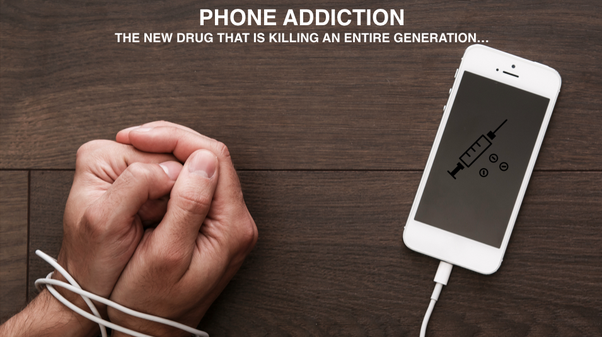
\includegraphics[scale=0.35]{ANGS3/addiction.png}
  \end{frame}
  
  \begin{frame}
  \hspace{1.5cm}
  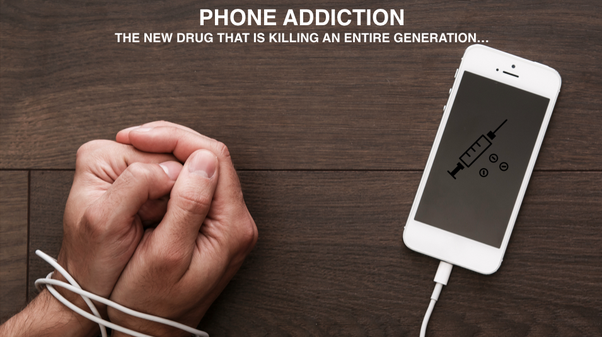
\includegraphics[scale=0.35]{ANGS3/addiction.png}
  \end{frame}
  
  \begin{frame}
  \hspace{1.5cm}
  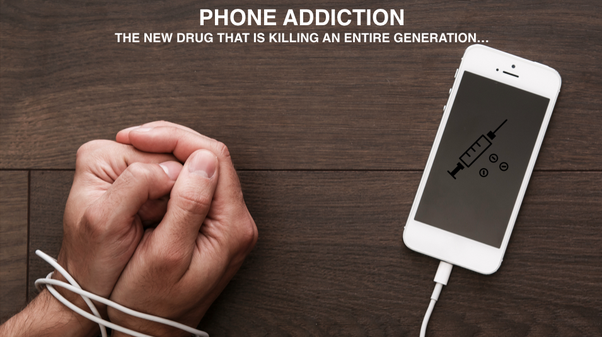
\includegraphics[scale=0.25]{ANGS3/addiction.png}
  \end{frame}
  
  \begin{frame} %1
	\hspace{1.7cm}
    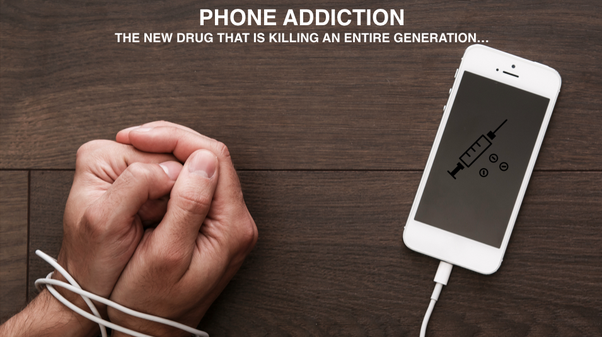
\includegraphics[scale=0.5]{ANGS3/addiction.png}
	
	\begin{exampleblock}{Exemple} 
	Alice choisit de cacher \textcolor{red}{message.txt} dans un fichier 
	BMP \textcolor{red}{photo.bmp} et veut obtenir le fichier 
	\textcolor{red}{piece\_jointe.bmp} après la 
	dissimulation. Enfin, elle choisit le mot de passe \textcolor{red}{alicebob}. 
	\end{exampleblock}
  \end{frame}
  
    \begin{frame} %3
	\begin{block}{Algorithmes de stéganographie}
	\begin{itemize}
	\setbeamertemplate{itemize item}[circle]
	\item Least Significant Bit (LSB)
	\item End Of File (EOF)
	\item Metadata
	\item End Of Chunk (EOC)
	\item Junk Chunk 
	\end{itemize}
	\end{block}
	
	\begin{alertblock}{Besoin} 
	Nécessité d'obtenir les informations de l'insertion pendant l'extraction
	impose une "signature".
	\end{alertblock}

  \end{frame}
  
  
  \begin{frame}
  
  \begin{block}{Signature StegX}
	\begin{itemize}
	\setbeamertemplate{itemize item}[circle]
	\item Identificateur de la méthode (1 octet).
	\item Identificateur de l'algorithme (1 octet). 
	\item Taille du fichier caché (4 octets). 
	\item Taille du nom du fichier caché (1 octet). 
	\item Nom du fichier caché (entre 1 et 255 octets). 
	\item Mot de passe (64 octets).  
	\end{itemize}
	\end{block}
  
  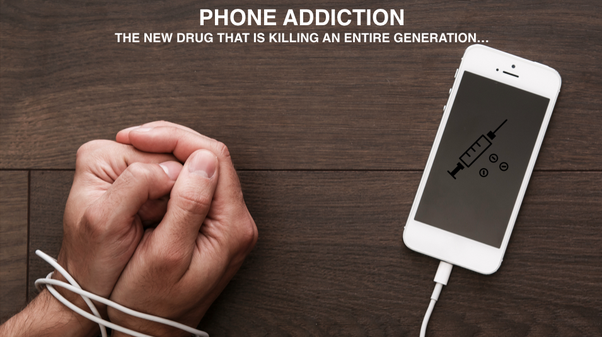
\includegraphics[scale=0.55]{ANGS3/addiction.png}
  \end{frame}
  
	% LSB OK
	\subsubsection{Least Significant Bit (LSB)}
	\begin{frame}
  
	\begin{block}{Least Significant Bit}
	\begin{itemize}
	\setbeamertemplate{itemize item}[circle]
	\item Modification des bits de poids faible des octets de données de 
	l'hôte. 
	\end{itemize}
	\end{block}
	
	\begin{exampleblock}{Avantage} 
	L'utilisation de cet algorithme n'augmente pas la taille du fichier 
	résultat en fonction de la taille du fichier caché. 
	\end{exampleblock}
	
	\begin{alertblock}{Inconvénient} 
	Le fichier à cacher doit être assez petit pour pouvoir le cacher intégralement 
	dans le fichier hôte. 
	\end{alertblock}
	
	\hspace{2.5cm}
    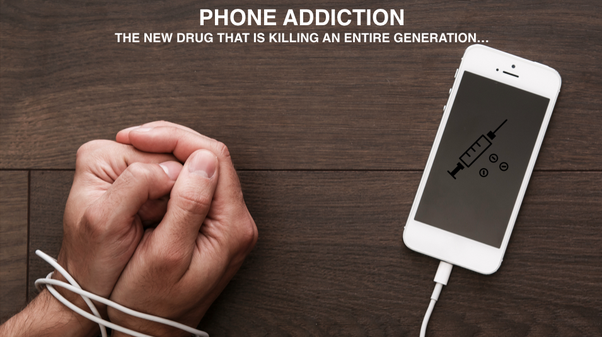
\includegraphics[scale=0.1]{ANGS3/addiction.png}
	\end{frame}
  
    \begin{frame}
    
	\begin{block}{End Of File}
	\begin{itemize}
	\setbeamertemplate{itemize item}[circle]
	\item Écriture des données à cacher après la fin officielle du fichier 
	hôte. 
	\end{itemize}
	\end{block}
	
	\begin{exampleblock}{Avantage} 
	Il n'y a pas de limite de taille pour cacher le fichier. 
	\end{exampleblock}
	
	\begin{alertblock}{Inconvénient} 
	L'utilisation de cet algorithme augmente considérablement la taille du 
	fichier résultat par rapport au fichier hôte. 
	\end{alertblock}
	
	\hspace{1cm}
    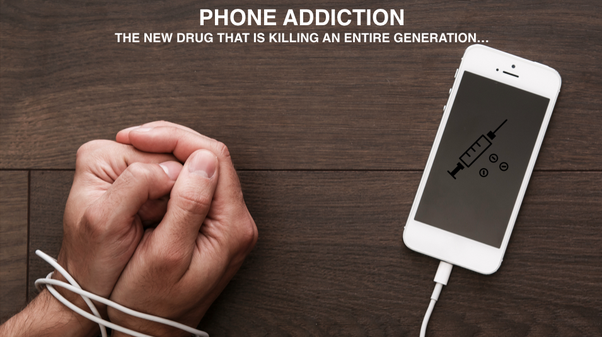
\includegraphics[scale=0.2]{ANGS3/addiction.png}
    
    \end{frame}
    
    % METADATA OK
    \begin{frame}
    
	\begin{block}{Metadata}
	\begin{itemize}
	\setbeamertemplate{itemize item}[circle]
	\item Écriture des données à cacher dans des blocs de données spécifiques 
	qui ne modifieront pas les données originales. 
	\end{itemize}
	\end{block}
	
	\begin{exampleblock}{Avantage} 
	Il n'y a pas de limite de taille pour cacher le fichier. 
	\end{exampleblock}
	
	\begin{alertblock}{Inconvénient} 
	L'utilisation de cet algorithme augmente considérablement la taille du 
	fichier résultat par rapport au fichier hôte. 
	\end{alertblock}
	
	\hspace{3.5cm}
    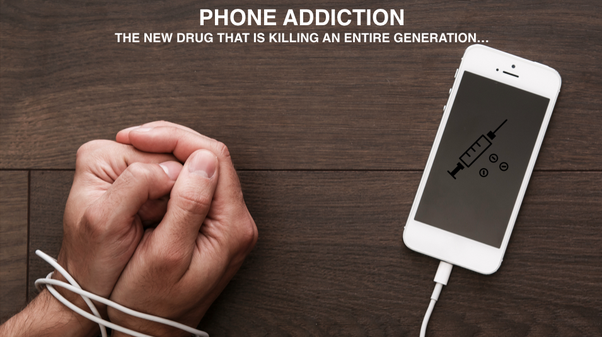
\includegraphics[scale=0.2]{ANGS3/addiction.png}
    
    \end{frame}
    
    \begin{frame}
    
	\begin{block}{End Of Chunk}
	\begin{itemize}
	\setbeamertemplate{itemize item}[circle]
	\item Écriture des données à cacher après les différents chunks interprétables 
	du fichier hôte. Ces données seront non reconnus et donc ignorés.  
	\end{itemize}
	\end{block}
	
	\begin{exampleblock}{Avantage} 
	Il n'y a pas de limite de taille pour cacher le fichier. 
	\end{exampleblock}
	
	\begin{alertblock}{Inconvénient} 
	L'utilisation de cet algorithme augmente considérablement la taille du 
	fichier résultat par rapport au fichier hôte. 
	\end{alertblock}
	
	\hspace{4.3cm}
    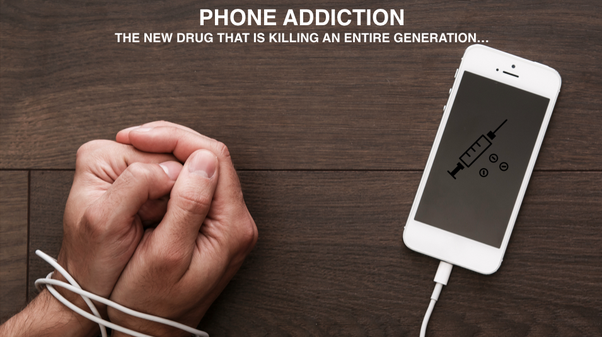
\includegraphics[scale=0.08]{ANGS3/addiction.png}
    
    \end{frame}
  
    \begin{frame}
    
	\begin{block}{Junk Chunk}
	\begin{itemize}
	\setbeamertemplate{itemize item}[circle]
	\item Écriture des données à cacher dans un chunk appelé "junk" : les 
	données ne seront pas interprétées  
	\end{itemize}
	\end{block}
	
	\begin{exampleblock}{Avantage} 
	Il n'y a pas de limite de taille pour cacher le fichier. 
	\end{exampleblock}
	
	\begin{alertblock}{Inconvénient} 
	L'utilisation de cet algorithme augmente considérablement la taille du 
	fichier résultat par rapport au fichier hôte. 
	\end{alertblock}
	
	\hspace{4.4cm}
    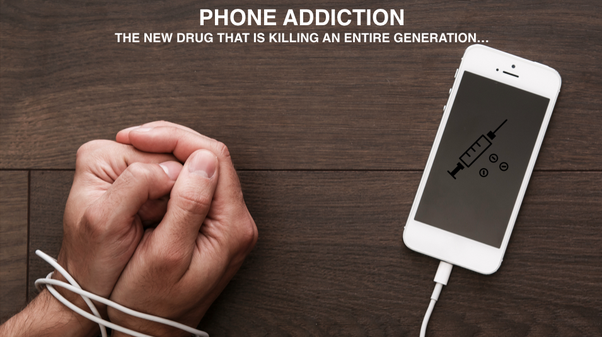
\includegraphics[scale=0.08]{ANGS3/addiction.png}
    
    \end{frame}

    \begin{frame} %1
	\begin{block}{Description des modules}
	\begin{itemize}
	\setbeamertemplate{itemize item}[circle]
	\item \textcolor{red}{Vérification de la compatibilité des fichiers.}
	\item \textcolor{gray} {Proposition des algorithmes de stéganographie.}
	\item \textcolor{gray} {Insertion des données.}
	\item \textcolor{gray} {Détection de l'algorithme de stéganographie.}
	\item \textcolor{gray} {Extraction des données.}
	\end{itemize}
	\end{block}
	
	\begin{exampleblock}{Exemple} 
	Avec la vérification de la compatibilité des fichiers, il s'agit d'un 
	format \textcolor{red}{BMP non compressé}.  
	\end{exampleblock}
  \end{frame}
  
  \begin{frame} %2
	\begin{block}{Description des modules}
	\begin{itemize}
	\setbeamertemplate{itemize item}[circle]
	\item Vérification de la compatibilité des fichiers.
	\item \textcolor{red}{Proposition des algorithmes de stéganographie.}
	\item \textcolor{gray} {Insertion des données.}
	\item \textcolor{gray} {Détection de l'algorithme de stéganographie.}
	\item \textcolor{gray} {Extraction des données.}
	\end{itemize}
	\end{block}
	
	\begin{exampleblock}{Exemple} 
	\begin{itemize}
	\setbeamertemplate{itemize item}[circle]
	\item Grâce au module Proposition des algorithmes de stéganographie, les 
	spécificités du format de piece\_jointe.bmp ont été déduites. 
	\item Les algorithmes \textcolor{red}{EOF}, \textcolor{red}{LSB} et 
	\textcolor{red}{Metadata} sont proposés. 
	\item Alice choisit l'algorithme \textcolor{red}{EOF}. 
	\end{itemize}
	
	\end{exampleblock}
  \end{frame}
  
  \begin{frame} %3
	\begin{block}{Description des modules}
	\begin{itemize}
	\setbeamertemplate{itemize item}[circle]
	\item Vérification de la compatibilité des fichiers.
	\item Proposition des algorithmes de stéganographie.
	\item \textcolor{red} {Insertion des données.}
	\item \textcolor{gray} {Détection de l'algorithme de stéganographie.}
	\item \textcolor{gray} {Extraction des données.}
	\end{itemize}
	\end{block}
	
	\begin{exampleblock}{Exemple} 
	Lors de l'insertion de Alice, l'algorithme EOF sera utilisé où 
	les données de l'hôte, la signature StegX suivies des données du fichier 
	à cacher seront écrites dans piece\_jointe.bmp. 
	\end{exampleblock}
  \end{frame}
  
  \begin{frame} %4
	\begin{block}{Description des modules}
	\begin{itemize}
	\setbeamertemplate{itemize item}[circle]
	\item Vérification de la compatibilité des fichiers.
	\item Proposition des algorithmes de stéganographie.
	\item Insertion des données.
	\item \textcolor{red} {Détection de l'algorithme de stéganographie.}
	\item \textcolor{gray} {Extraction des données.}
	\end{itemize}
	\end{block}
	
		\begin{exampleblock}{Exemple} 
	Après que Alice ait fini la dissimulation, Bob va déduire les spécificités
	du fichier piece\_jointe.bmp et déduire les informations sur le fichier 
	caché message.txt. 
	\end{exampleblock}
  \end{frame}
  
  \begin{frame} %5
	\begin{block}{Description des modules}
	\begin{itemize}
	\setbeamertemplate{itemize item}[circle]
	\item Vérification de la compatibilité des fichiers.
	\item Proposition des algorithmes de stéganographie.
	\item Insertion des données.
	\item Détection de l'algorithme de stéganographie.
	\item \textcolor{red}{Extraction des données.}
	\end{itemize}
	\end{block}
	
	\begin{exampleblock}{Exemple} 
	L'algorithme EOF sera utilisé pour extraire les  données du fichier 
	caché de message.txt. 
	\end{exampleblock}
  \end{frame}
  
  \begin{frame}
	\begin{alertblock}{Problème} 
	Si Oscar connaît la stéganographie, il peut utiliser un éditeur 
	hexadécimal en voir en clair les données cachées.
	\end{alertblock}
	
	\begin{exampleblock}{Solution} 
	L'utilisation d'une méthode de protection des données est ajoutée : 
	 \begin{itemize}
	 \setbeamertemplate{itemize item}[circle]
	\item Données à cacher XORées avec une suite pseudo-aléatoire générée
	à partir du mot de passe (chiffrement par substitution polyalphabétique).
	\item Données à cacher mélangées (chiffrement par transposition).
	\end{itemize}
	\end{exampleblock}
  \end{frame}
  
   
  
  \begin{frame}
  
	\begin{block}{Lecture et écriture de fichiers : endianness en fonction des formats}
	\begin{itemize}
	\setbeamertemplate{itemize item}[circle]

	\item Little endian et big endian selon les formats. 
	\item Travail de recherche poussé pour chaque format et pour chaque 
	algorithme de stéganographie.
	\end{itemize}
	\end{block}
		
	\begin{block}{Format MP3}
	\begin{itemize}
	\setbeamertemplate{itemize item}[circle]
	\item Format compressé utilisant des algorithmes de compression complexes.
	\item Étude des versions des formats (MPEG 1 Layer III, MPEG 2 Layer III). 
	\item Étude des versions de formats de métadonnée (ID3 version 1, ID3 version 2). 
	\end{itemize}
	\end{block}
	
	\end{frame}
  
  
  \begin{frame}
  
	\begin{block}{Bilan logiciel}
	\begin{itemize}
	\setbeamertemplate{itemize item}[circle]
	\item Faire de la stéganographie sur des fichiers image, audio et vidéo
	(insertion et extraction). \checkmark
	\item Plusieurs formats sont gérés et une diversité dans les algorithmes 
	sont proposés. \checkmark
	\item Réaliser deux interfaces : ligne de commande et graphique. \checkmark
\setbeamertemplate{itemize item}[triangle]
	\item Futures améliorations : nouveaux formats et algorithmes. 

\end{itemize}
	
	\end{block}
	
	\begin{block}{Bilan humain}
	\begin{itemize}
	\setbeamertemplate{itemize item}[circle]
	\item L'équipe s'est efforcée à travailler de façon professionnelle et ordonnée.
	\item Projet de grande envergure qui a nécessité de diviser la conception 
	selon les trois types de formats étudiés.  
	\end{itemize}
	\end{block}

	\end{frame}
  
\end{document}
